\documentclass[tikz,border=5pt]{standalone}
\usepackage{times}
\usepackage{amsmath,amssymb}
\usetikzlibrary{positioning,fit,arrows.meta,backgrounds,shapes.geometric,calc,shadows,decorations.pathreplacing}

\begin{document}
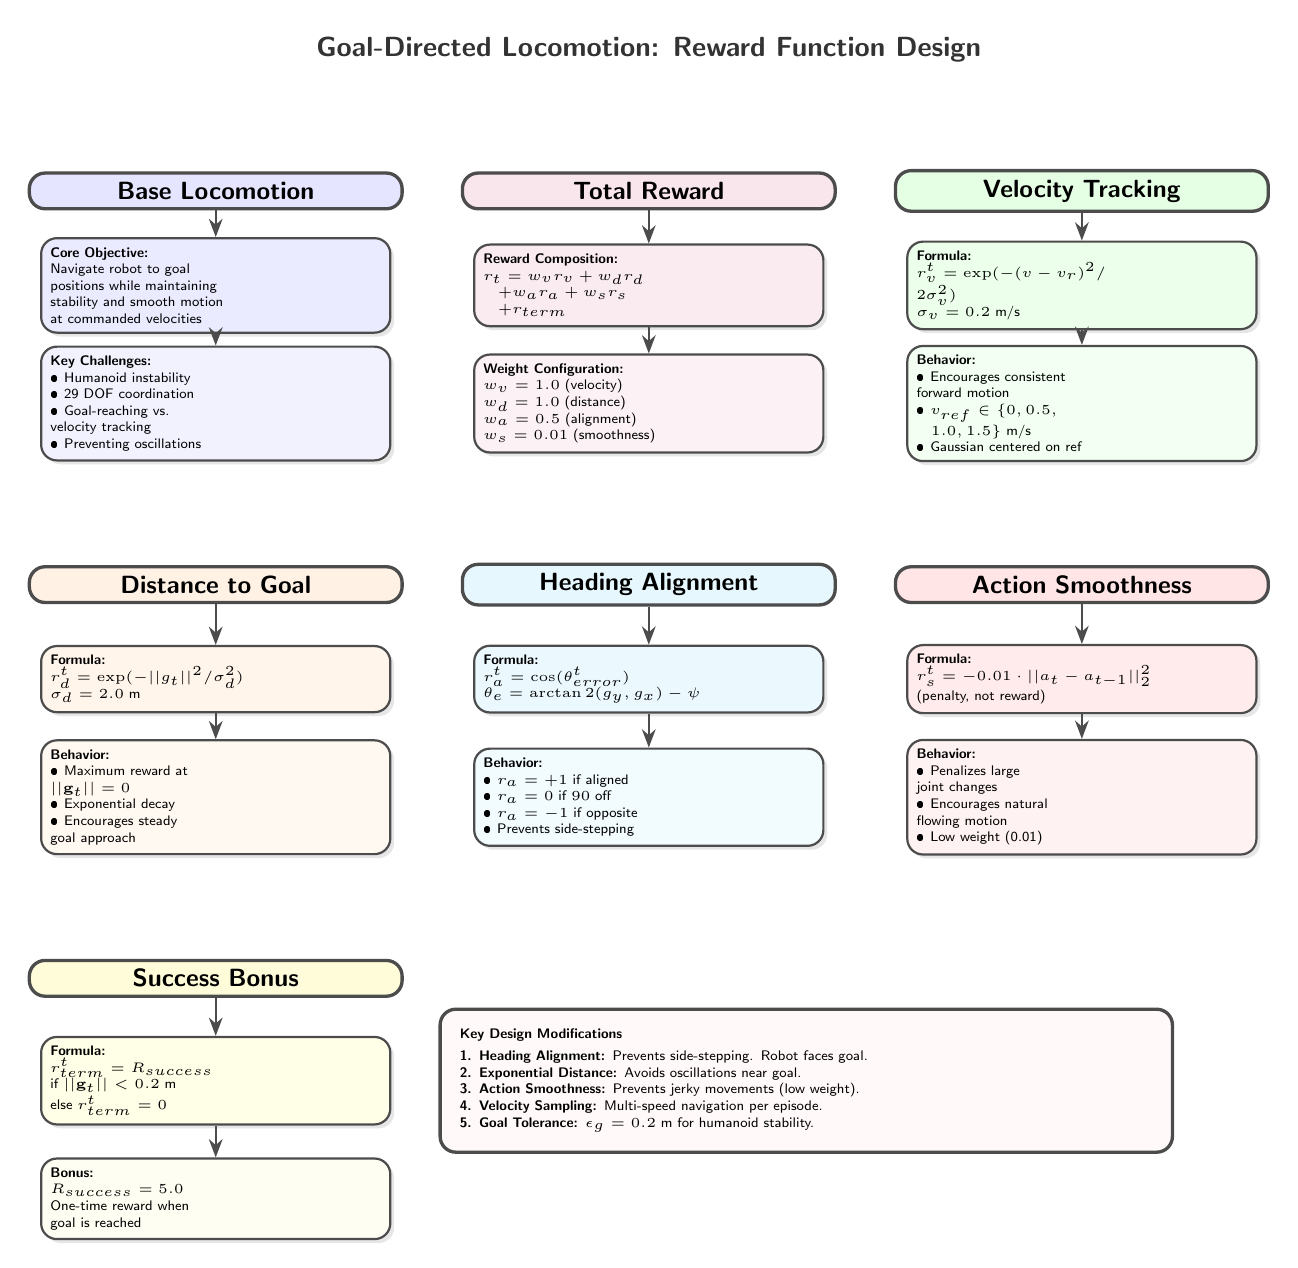
\begin{tikzpicture}[
    node distance=1.0cm and 1.3cm,
    box/.style={
        draw=black!70,
        rounded corners=2mm,
        fill=white,
        thick,
        font=\sffamily\small,
        align=center,
        drop shadow={opacity=0.2, shadow xshift=0.05cm, shadow yshift=-0.05cm}
    },
    header/.style={
        font=\sffamily\bfseries\normalsize,
        color=black!80
    },
    formula/.style={
        font=\ttfamily\footnotesize,
        color=black!70
    },
    arrow/.style={->, >=Stealth, thick, color=black!70},
    label/.style={font=\sffamily\tiny, color=black!60}
]

% ============================================================
% TITLE
% ============================================================
\node[header] at (7.5, 13.8) {Goal-Directed Locomotion: Reward Function Design};

% ============================================================
% BASE LOCOMOTION PRINCIPLES (TOP-LEFT)
% ============================================================
\node[draw=black!70, rounded corners=2mm, fill=blue!10, very thick, text width=4.5cm, align=center, font=\sffamily\small] (base_header) at (2.0, 12.0) {\textbf{Base Locomotion}};

\node[box, fill=blue!8, text width=4.2cm, font=\sffamily\tiny, align=left] (base_principle) at (2.0, 10.8) {
\textbf{Core Objective:}\\
Navigate robot to goal\\
positions while maintaining\\
stability and smooth motion\\
at commanded velocities
};

\node[box, fill=blue!5, text width=4.2cm, font=\sffamily\tiny, align=left] (base_challenge) at (2.0, 9.3) {
\textbf{Key Challenges:}\\
• Humanoid instability\\
• 29 DOF coordination\\
• Goal-reaching vs.\\
  velocity tracking\\
• Preventing oscillations
};

\draw[arrow] (base_header) -- (base_principle);
\draw[arrow] (base_principle) -- (base_challenge);

% ============================================================
% REWARD COMPOSITION (CENTER-TOP)
% ============================================================
\node[draw=black!70, rounded corners=2mm, fill=purple!10, very thick, text width=4.5cm, align=center, font=\sffamily\small] (reward_total_header) at (7.5, 12.0) {\textbf{Total Reward}};

\node[box, fill=purple!8, text width=4.2cm, font=\sffamily\tiny, align=left] (reward_total_eq) at (7.5, 10.8) {
\textbf{Reward Composition:}\\
$r_t = w_v r_v + w_d r_d$\\
$\quad + w_a r_a + w_s r_s$\\
$\quad + r_{term}$
};

\node[box, fill=purple!5, text width=4.2cm, font=\sffamily\tiny, align=left] (reward_weights) at (7.5, 9.3) {
\textbf{Weight Configuration:}\\
$w_v = 1.0$ (velocity)\\
$w_d = 1.0$ (distance)\\
$w_a = 0.5$ (alignment)\\
$w_s = 0.01$ (smoothness)
};

\draw[arrow] (reward_total_header) -- (reward_total_eq);
\draw[arrow] (reward_total_eq) -- (reward_weights);

% ============================================================
% VELOCITY TRACKING (TOP-RIGHT)
% ============================================================
\node[draw=black!70, rounded corners=2mm, fill=green!10, very thick, text width=4.5cm, align=center, font=\sffamily\small] (vel_header) at (13.0, 12.0) {\textbf{Velocity Tracking}};

\node[box, fill=green!8, text width=4.2cm, font=\sffamily\tiny, align=left] (vel_formula) at (13.0, 10.8) {
\textbf{Formula:}\\
$r_v^t = \exp(-(v - v_r)^2/$\\
$2\sigma_v^2)$\\
$\sigma_v = 0.2$ m/s
};

\node[box, fill=green!5, text width=4.2cm, font=\sffamily\tiny, align=left] (vel_behavior) at (13.0, 9.3) {
\textbf{Behavior:}\\
• Encourages consistent\\
  forward motion\\
• $v_{ref} \in \{0, 0.5,$\\
$\quad 1.0, 1.5\}$ m/s\\
• Gaussian centered on ref
};

\draw[arrow] (vel_header) -- (vel_formula);
\draw[arrow] (vel_formula) -- (vel_behavior);

% ============================================================
% DISTANCE TO GOAL (MIDDLE-LEFT)
% ============================================================
\node[draw=black!70, rounded corners=2mm, fill=orange!10, very thick, text width=4.5cm, align=center, font=\sffamily\small] (dist_header) at (2.0, 7.0) {\textbf{Distance to Goal}};

\node[box, fill=orange!8, text width=4.2cm, font=\sffamily\tiny, align=left] (dist_formula) at (2.0, 5.8) {
\textbf{Formula:}\\
$r_d^t = \exp(-||g_t||^2 / \sigma_d^2)$\\
$\sigma_d = 2.0$ m
};

\node[box, fill=orange!5, text width=4.2cm, font=\sffamily\tiny, align=left] (dist_behavior) at (2.0, 4.3) {
\textbf{Behavior:}\\
• Maximum reward at\\
  $||\mathbf{g}_t|| = 0$\\
• Exponential decay\\
• Encourages steady\\
  goal approach
};

\draw[arrow] (dist_header) -- (dist_formula);
\draw[arrow] (dist_formula) -- (dist_behavior);

% ============================================================
% HEADING ALIGNMENT (MIDDLE-CENTER)
% ============================================================
\node[draw=black!70, rounded corners=2mm, fill=cyan!10, very thick, text width=4.5cm, align=center, font=\sffamily\small] (head_header) at (7.5, 7.0) {\textbf{Heading Alignment}};

\node[box, fill=cyan!8, text width=4.2cm, font=\sffamily\tiny, align=left] (head_formula) at (7.5, 5.8) {
\textbf{Formula:}\\
$r_a^t = \cos(\theta_{error}^t)$\\
$\theta_e = \arctan2(g_y, g_x) - \psi$
};

\node[box, fill=cyan!5, text width=4.2cm, font=\sffamily\tiny, align=left] (head_behavior) at (7.5, 4.3) {
\textbf{Behavior:}\\
• $r_a = +1$ if aligned\\
• $r_a = 0$ if $90°$ off\\
• $r_a = -1$ if opposite\\
• Prevents side-stepping
};

\draw[arrow] (head_header) -- (head_formula);
\draw[arrow] (head_formula) -- (head_behavior);

% ============================================================
% ACTION SMOOTHNESS (MIDDLE-RIGHT)
% ============================================================
\node[draw=black!70, rounded corners=2mm, fill=red!10, very thick, text width=4.5cm, align=center, font=\sffamily\small] (smooth_header) at (13.0, 7.0) {\textbf{Action Smoothness}};

\node[box, fill=red!8, text width=4.2cm, font=\sffamily\tiny, align=left] (smooth_formula) at (13.0, 5.8) {
\textbf{Formula:}\\
$r_s^t = -0.01 \cdot ||a_t - a_{t-1}||_2^2$\\
(penalty, not reward)
};

\node[box, fill=red!5, text width=4.2cm, font=\sffamily\tiny, align=left] (smooth_behavior) at (13.0, 4.3) {
\textbf{Behavior:}\\
• Penalizes large\\
  joint changes\\
• Encourages natural\\
  flowing motion\\
• Low weight (0.01)
};

\draw[arrow] (smooth_header) -- (smooth_formula);
\draw[arrow] (smooth_formula) -- (smooth_behavior);

% ============================================================
% SUCCESS BONUS (BOTTOM-LEFT)
% ============================================================
\node[draw=black!70, rounded corners=2mm, fill=yellow!15, very thick, text width=4.5cm, align=center, font=\sffamily\small] (success_header) at (2.0, 2.0) {\textbf{Success Bonus}};

\node[box, fill=yellow!10, text width=4.2cm, font=\sffamily\tiny, align=left] (success_formula) at (2.0, 0.7) {
\textbf{Formula:}\\
$r_{term}^t = R_{success}$\\
if $||\mathbf{g}_t|| < 0.2$ m\\
else $r_{term}^t = 0$
};

\node[box, fill=yellow!5, text width=4.2cm, font=\sffamily\tiny, align=left] (success_behavior) at (2.0, -0.8) {
\textbf{Bonus:}\\
$R_{success} = 5.0$\\
One-time reward when\\
goal is reached
};

\draw[arrow] (success_header) -- (success_formula);
\draw[arrow] (success_formula) -- (success_behavior);

% ============================================================
% DESIGN MODIFICATIONS (BOTTOM-CENTER & RIGHT)
% ============================================================
\node[draw=black!70, rounded corners=2mm, fill=pink!10, very thick, text width=8.8cm, align=left, font=\sffamily\tiny, inner sep=0.25cm] (modifications_box) at (9.5, 0.7) {
\textbf{Key Design Modifications}\\[2pt]
\textbf{1. Heading Alignment:} Prevents side-stepping. Robot faces goal.\\
\textbf{2. Exponential Distance:} Avoids oscillations near goal.\\
\textbf{3. Action Smoothness:} Prevents jerky movements (low weight).\\
\textbf{4. Velocity Sampling:} Multi-speed navigation per episode.\\
\textbf{5. Goal Tolerance:} $\epsilon_g = 0.2$ m for humanoid stability.
};

\end{tikzpicture}
\end{document}
